%------------------------------------------------------------------------------
% A template for using the SVNITPhDThesis.cls class file. 
% author : Milind Padalkar (milind.padalkar@gmail.com)
% modified for M.Tech by : Shreyas Patel (shreyaspate29@gmail.com)

%------------------------------------------------------------------------------
\documentclass{SVNITPhDReport}
%------------------------------------------------------------------------------
%Preamble
%Do not omit the following fields
%------------------------------------------------------------------------------

%Seminar Type
\seminarType{Report}

%Author title. Valid entries : Mr. Ms. Mrs.
\atitle{Mr.} 

%Author name
\author{YourName} 

%Report title
\title{ProjectTitle} 

%Department name
\dept{Computer Engineering}

%Registration number 
\regno{RollNo} 

%Supervisor title. Examples : Dr. Prof.
\stitleI{Dr.}
\supervisorI{InternalGuideName}
\sinstI{SVNIT}
\scityI{Surat}

\stitleII{Dr.}
\supervisorII{ExternalGuideName}
\sinstII{CompanyName}
\scityII{Mumbai}

\hodtitle{Prof.}
\hodname{HODNAME}

%Institute name
\addressInstN{Sardar Vallabhbhai National}
\addressInstD{Institute of Technology}
\addressInstP{Surat} 

%Month
\acMonth{December}

%Academic Year
\acYear{2015-- 2016}

%Calander Year
\calYear{2015}

%Institute logo file		
\instlogo{./Figures/logo}

%Path to border-style page
\borderPath{./Figures/border}

%------------------------------------------------------------------------------
%Preamble Ends here
%------------------------------------------------------------------------------

% User packages
\usepackage[numbers,sort&compress]{natbib}
\renewcommand{\bibfont}{\footnotesize}
\setlength{\bibsep}{5pt}

% User packages (You can add as many as you want)
\usepackage{amssymb}  %  for double struck characters
\usepackage{subfigure} % for subfigures
\usepackage{enumerate}
\usepackage{algorithm}
\usepackage{algorithmic}
\usepackage{listings}
\usepackage{fancybox}
\usepackage{makeidx}  % allows for indexgeneration
\usepackage{graphicx} % for adding figures
\usepackage{amsmath}
\usepackage{booktabs}
\usepackage{ctable}
\usepackage{float}
\usepackage{stmaryrd}
\usepackage{listings}
\usepackage{fancybox}
\usepackage{txfonts}
\usepackage{subfigure}
\usepackage{rotating}
\usepackage{tabularx}
\usepackage{longtable} % also needed by longtabu
\usepackage{tabu}
\usepackage{multirow}
\usepackage{booktabs}
\usepackage{upgreek}
\usepackage{tipa} 
\usepackage{color}
%\usepackage{fontenc}
\usepackage[titletoc]{appendix}
\usepackage{url}
\usepackage{acronym}
\usepackage{wrapfig}
\usepackage{lscape}
\usepackage{rotating}
\usepackage{pbsi}
\usepackage[T1]{fontenc}
\usepackage{calligra} 
\usepackage{fancyhdr}
\usepackage{natbib}
\usepackage[english]{babel}
\usepackage{afterpage}

\begin{document}
%%Create the title page
\addpageborder	
\maketitle

%assign page number
\pagenumbering{roman}
\setcounter{page}{2}

%%Create the declaration page
\putdecleration

%%Create the certificate page
%\putcertificate

\putnewcertificate

%Create the acknowledgement page
%\addcontentsline{toc}{chapter}{Acknowledgements} 
\putsvnitack
%{\label{sec:ack}

	\textit{		
		\hspace*{10pt} At the outset, I thank the God Almighty for the grace, strength and hope to make my endeavor a success. I express my sincere gratitude to my guides \@stitleI \@supervisorI, Assistant Professor, Computer Engineering Department, SVNIT and \@stitleII \@supervisorII, Principal Technical Officer, Electronics and Information Technology Department, C-DAC, Mumbai for their exemplary guidance, monitoring and constant encouragement without which the successful completion of this report would not have been possible.
		\\
	}

	\textit{
		\hspace*{10pt} I am also highly grateful to the staff of Computer Department for giving me a lot of their valuable time, as well as guidance and suggestions whenever I needed them.
		\\
	}
	
	\textit{
		\hspace*{10pt} I would like to thank to my friends, who stood by me, whenever I needed their assistance and also gave me the strengths to carry on.
		\\
	}

	\textit{
		\hspace*{10pt} I would like to express my gratitude towards my parents and family for their kind co-operation and encouragement which help me completion of my seminar work.	
	}}

%Create the abstract page
%\newpage
\putsvnitabstract{
\label{sec:abstract}

\textit{
	Your abstract goes here . . .
}

\vspace{10pt}
}

%Create the table of contents page
\bordertoc

%Create the Bordered LoF page
\addcontentsline{toc}{section}{List of Figures} % Entry in ToC
\borderlof

%Create the Bordered LoT page
%\addcontentsline{toc}{section}{List of Tables} % Entry in ToC
%\borderlot

%List of Acronyms
%\addcontentsline{toc}{section}{List of Acronyms} % Entry in ToC
%\label{page:Acronyms}
\begin{center}
	\textbf{\Large List of Acronyms}
\end{center}

%\section*{List of Acronyms}
%\begin{acronym}
%	\acro{WSN} Wireless Sensor Network\vspace*{0.5mm}
%\end{acronym}
\newpage

%\addcontentsline{toc}{section}{List of Symbols} % Entry in ToC
%\label{page:Symbols}
\begin{center}
\textbf{\Large List of Symbols}
\end{center}
%{$K_{t}$}\hspace{10mm}{Kalman Gain}\\
%{$x_{t}$}\hspace{11mm}{State Vector}\\
%{$P_{t}$}\hspace{10mm}{Updated Estimate Covariance}
\newpage

\clearpageborder

\setcounter{page}{1}
\pagenumbering{arabic}
\lhead{}
\setlength{\headheight}{15.2pt}
\pagestyle{fancy}
\chapter{Introduction}

Chapter 1 contents goes here . . . 

\section{Section 1}
	
	This is section  . . . 

	\subsection{Sub Section}

		This is sub sub section  . . . 


		Here is the example of bullets

		\begin{itemize}

			\item Item 1 \\
			Item 1 content goes here . . .

			\item Item 2 \\
			Item 2 content goes here . . .


		\end{itemize}

		Here is the example of enumerated bullets . . . You can replace [A.] with [a.] . . .

		\begin{enumerate}[A.]

		\item Item 1 \\
			Item 1 content goes here . . .

			\item Item 2 \\
			Item 2 content goes here . . .

		\end{enumerate}

\newpage %Introduction
\blankpage
\chapter {Theoretical Background \& Literature Survey}

Chapter 2 content goes here ...

\section{Car}

	Figure ~\ref{fig:CarExample} shows example of how to add image in latex . . .

	\begin{figure}[h]
		\begin{center}
  			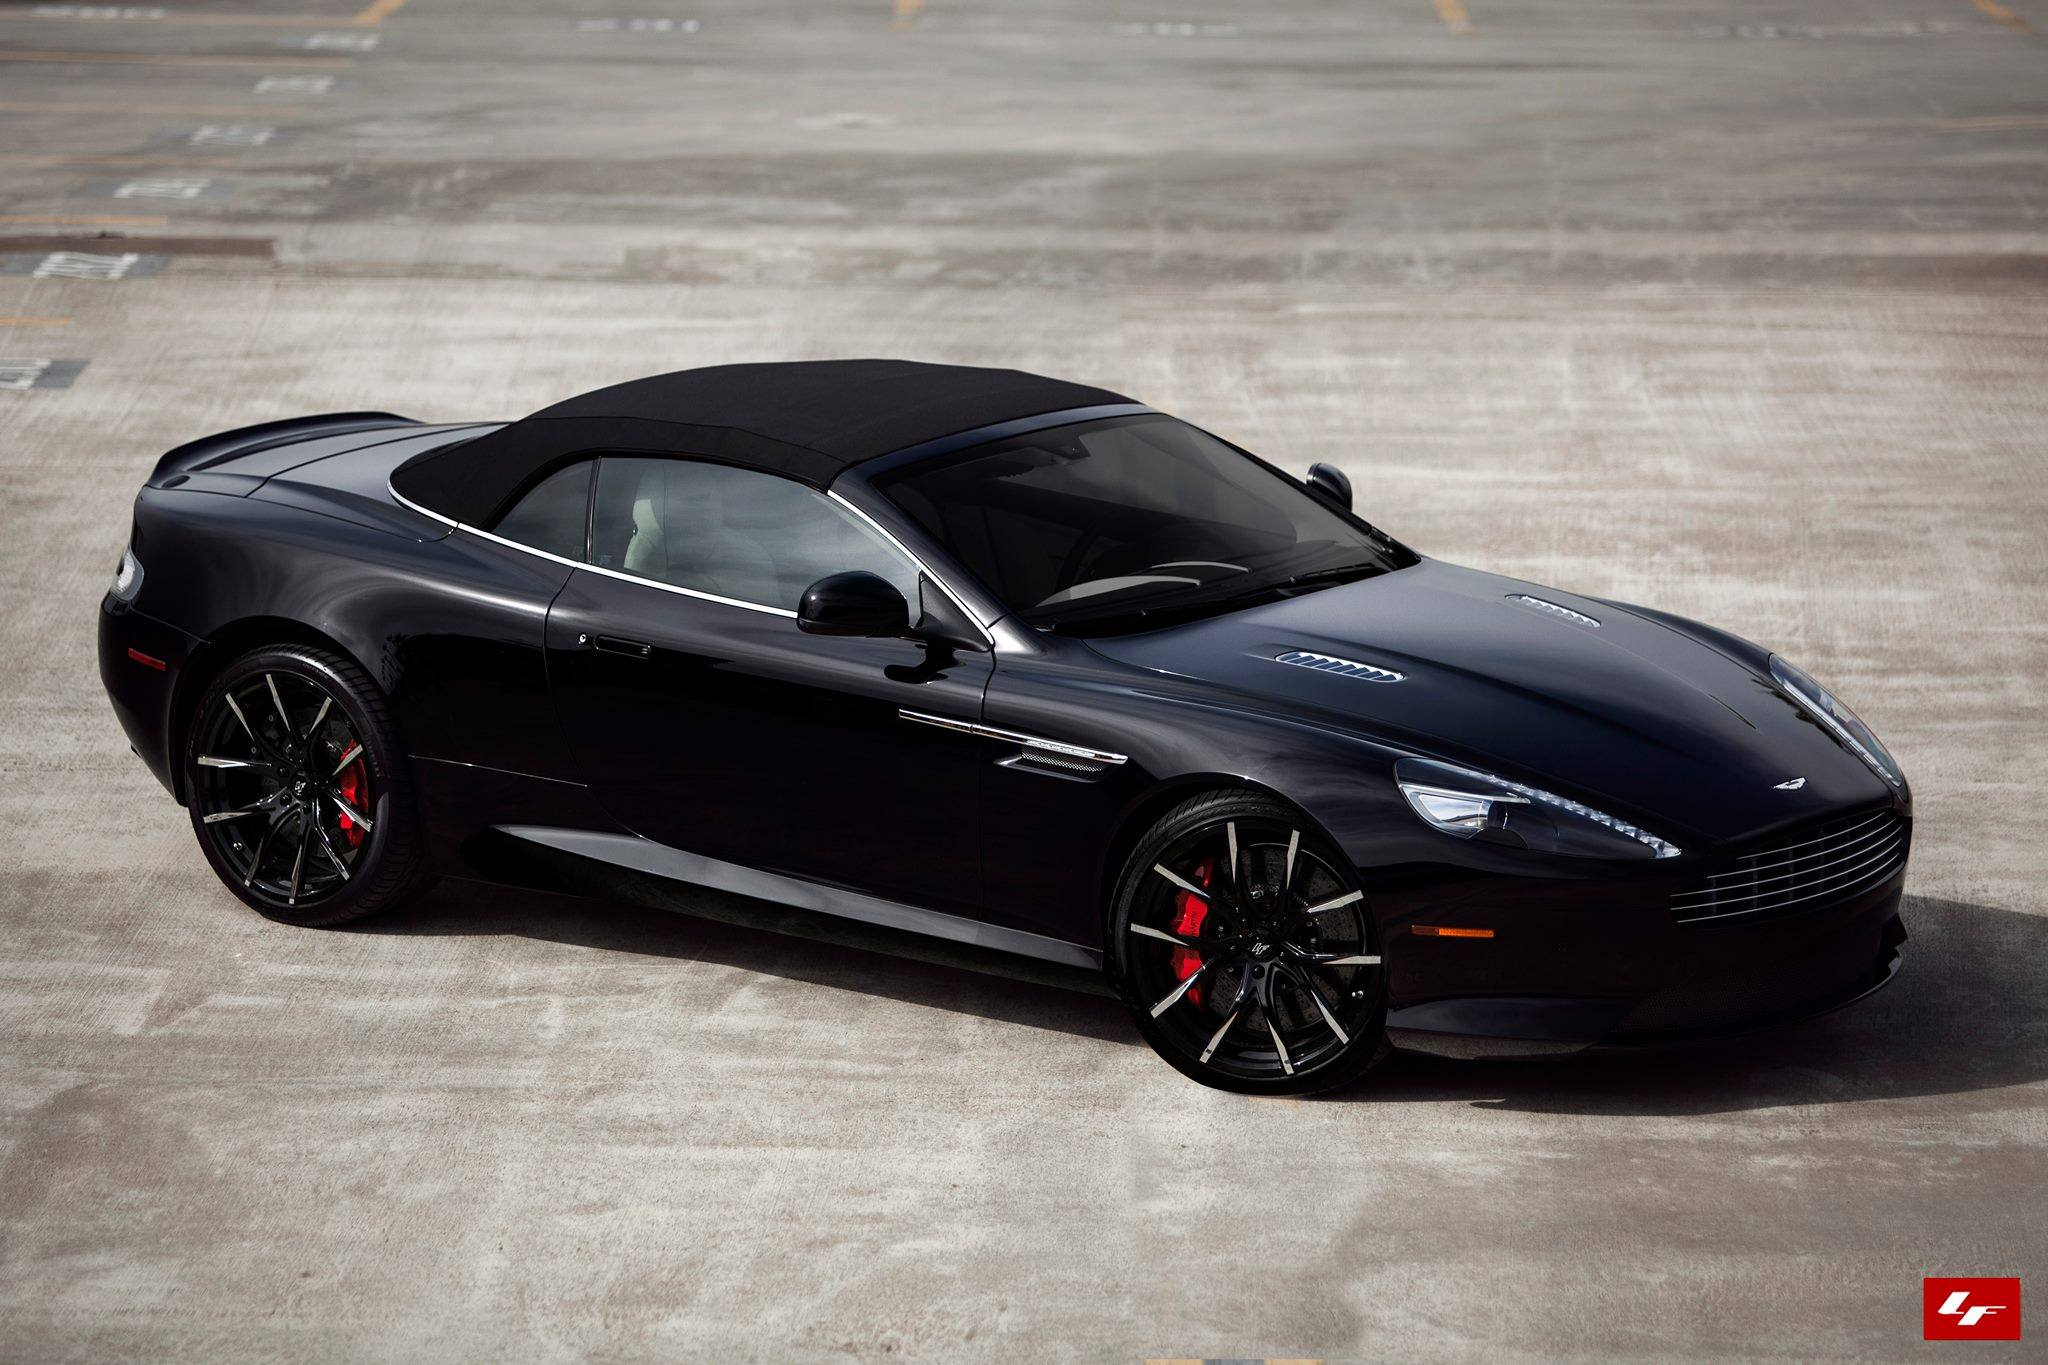
\includegraphics[width=3in,keepaspectratio]{./Chapter2/Chapter2Figs/car.jpg}\\
				\caption[My Car]{My Car \cite{BibLabel}}
				\label{fig:CarExample}
		\end{center}
	\end{figure}

\section{Add Table}
	If you want to add table use http://www.tablesgenerator.com/ web-site.}
 %Theoretical Background & Literature survey
\blankpage
%Include Appendix
%\begin{appendices}
\chapter{Classical Multi-Dimensional Scaling}
In the Classical MDS it is assumed that, there is a linear relationship between Euclidean distance and shortest path distance between each pair of nodes. For each pair of nodes $(i,j)$, if the Euclidean distance and shortest path are denoted by $d_{ij}$, and $p_{ij}$ respectively; then the relation between $d_{ij}$ and $p_{ij}$ can be represented as $d_{ij}=kp_{ij}+c$, where $k$ and $c$ are constants.
Let the $n$ number of nodes are deployed on the field. The coordinates of $n$ points in a $m$ dimensional Euclidean space be given by $X_{i}=(x_{i1},....,x_{im})^{T}$,
Then the squared Euclidean distance between the $i^{th}$ and $j^{th}$ nodes is defined by -
\begin{displaymath}
d^{2}_{ij} = {\sum\limits_{a=1}^m (X_{ia}-X_{ja})^2}=
 {\sum\limits_{a=1}^m X_{ia}^{2}+ X_{ja}^{2}-2X_{ia}X_{ja}}
\label{300}
\end{displaymath}
Let $D^{2}(X)$ denote the matrix of squared distances. For example, when $X$ contains the coordinates of three points in two dimensions, $D^{2}(X)$ can be represented as-
\begin{displaymath}
D^{2}(X) =
\left( \begin{array}{ccccc}
0 & d_{12}^2 & d_{13}^2 & \ldots & d_{1n} \\
d_{12}^2 & 0 & d_{23}^2 & \ldots & d_{2n}\\
\vdots & \vdots & \vdots & \ldots & \vdots \\
d_{1n}^2 & d_{2n}^2 & d_{3n}^2 & \ldots & 0 \\
\end{array} \right)	\\
\end{displaymath}
\begin{displaymath}
= \sum\limits_{a=1}^2{\left( \begin{array}{ccccc}
x_{1a}^2 & x_{1a}^2 & \ldots & x_{1a}^2 \\
x_{2a}^2 & x_{2a}^2 & \ldots & x_{2a}^2 \\
\vdots   & \ddots   &        & \vdots\\
x_{na}^2 & x_{na}^2 & \ldots & x_{na}^2 \\
\end{array} \right)	}+
\sum\limits_{a=1}^2{\left( \begin{array}{ccccc}
x_{1a}^2 & x_{2a}^2 & \ldots & x_{na}^2 \\
x_{1a}^2 & x_{2a}^2 & \ldots & x_{na}^2 \\
\vdots   & \ddots   &        & \vdots\\
x_{1a}^2 & x_{2a}^2 & \ldots & x_{na}^2 \\
\end{array} \right)	} 
-
2{\sum\limits_{a=1}^2{\left( \begin{array}{ccccc}
x_{1a}^2 x_{1a}^2& x_{1a}^2 x_{2a}^2 & \ldots & x_{1a}^2x_{na}^2 \\
x_{2a}^2 x_{1a}^2 & x_{2a}^2 x_{2a}^2 & \ldots & x_{2a}^2 x_{na}^2\\
\vdots   & \ddots   &        & \vdots\\
x_{na}^2 x_{1a}^2& x_{na}^2 x_{2a}^2& \ldots & x_{na}^2x_{na}^2 \\
\end{array} \right)	}}
\end{displaymath}
Where, diagonal elements $x^{2}_{ij}$ for $i=j$ are 0.\\

\end{appendices}
\newpage
%Include Bibliography
%\rhead{\textit{Bibliography}}
\addcontentsline{toc}{chapter}{Bibliography}
\bibliographystyle{ieeetr}
%\renewcommand{\bibname}{\bibname}
\bibliography{SVNITPhDbibtex}

%\rhead{\textit{List of Publications}}
%\addcontentsline{toc}{chapter}{List of Publications} % Entery in ToC
%\label{page:pub}
\begin{center}
\textbf{\Large List of Publications}
\end{center}
\vspace*{25pt}
\begin{enumerate}[{[1]}]

\item S. Patil, A. Gupta, and M. Zaveri, ``Recovery of lost target in Wireless Sensor Network,'' \textit{submitted in EURASIP Journal on Wireless Communications and Networking}, (Revised Manuscript submitted).

\item S. Patil, A. Gupta, and M. Zaveri, ``Efficient target recovery in wireless sensor network,” \textit{in Advances in Computing and Information Technology}, ser. Advances in Intelligent Systems and Computing, Springer Berlin Heidelberg, 2012, vol. 176, pp. 385 – 394.

\item S. Patil, A. Gupta, and M. Zaveri, ``Localization in wireless sensor network: A distributed approach,” \textit{in Advances in Computing and Information Technology}, ser. Advances in Intelligent Systems and Computing, Springer Berlin Heidelberg, 2012, vol. 176, pp. 467-476.

\item A. Gupta, S. Patil, and M. Zaveri, ``Lost Target Recovery in Wireless Sensor Network Using Tracking,'' \textit{in proceedings of IEEE International Conference on Communication Systems and Network Technologies (CSNT)}. Rajkot,India: IEEE, May 2012, pp. 352–356.

\item S. Patil, and M. Zaveri, ``Localization in Wireless sensor Network with Nystrom Approximation,'' \textit{in International Journal of Wireless and Mobile Communication}, 3(5),Oct 2011, pp.37-48

\item S. Patil, and M. Zaveri, ``MDS and Trilateration based Localization in Wireless Sensor Network,'' \textit{in International Journal of Wireless Sensor Network, Scientific Research}, USA, 3(6), 2011, pp.198-208

\item S. Patil, and M. Zaveri, ``Energy efficient localization in Sensor network,'' \textit{in proceedings of IEEE International conference of HiPC 2011, (WonGen 2011)}, Banglore, 18-21 Dec. 2011

\item S. Patil, and M. Zaveri, ``Target Tracking approaches in Wireless sensor Network,'' \textit{in Proceedings of Computer Communication and Network, (CCN10)}, Florida, USA, 12-14 July 2010, pp.130-137

\end{enumerate}

\newpage
\nocite{timepass}
\end{document}